% (find-LATEX "2021-1-C2-intro.tex")
% (defun c () (interactive) (find-LATEXsh "lualatex -record 2021-1-C2-intro.tex" :end))
% (defun C () (interactive) (find-LATEXsh "lualatex 2021-1-C2-intro.tex" "Success!!!"))
% (defun D () (interactive) (find-pdf-page      "~/LATEX/2021-1-C2-intro.pdf"))
% (defun d () (interactive) (find-pdftools-page "~/LATEX/2021-1-C2-intro.pdf"))
% (defun e () (interactive) (find-LATEX "2021-1-C2-intro.tex"))
% (defun o () (interactive) (find-LATEX "2021-1-C2-intro.tex"))
% (defun u () (interactive) (find-latex-upload-links "2021-1-C2-intro"))
% (defun v () (interactive) (find-2a '(e) '(d)))
% (defun d0 () (interactive) (find-ebuffer "2021-1-C2-intro.pdf"))
% (defun cv () (interactive) (C) (ee-kill-this-buffer) (v) (g))
%          (code-eec-LATEX "2021-1-C2-intro")
% (find-pdf-page   "~/LATEX/2021-1-C2-intro.pdf")
% (find-sh0 "cp -v  ~/LATEX/2021-1-C2-intro.pdf /tmp/")
% (find-sh0 "cp -v  ~/LATEX/2021-1-C2-intro.pdf /tmp/pen/")
%     (find-xournalpp "/tmp/2021-1-C2-intro.pdf")
%   file:///home/edrx/LATEX/2021-1-C2-intro.pdf
%               file:///tmp/2021-1-C2-intro.pdf
%           file:///tmp/pen/2021-1-C2-intro.pdf
% http://angg.twu.net/LATEX/2021-1-C2-intro.pdf
% (find-LATEX "2019.mk")
% (find-CN-aula-links "2021-1-C2-intro" "2" "c2m211intro" "c2i")
%
% Video:
% (find-ssr-links "c2m211intro" "2021-1-C2-intro" "AIv4N8go1Bg")
% (code-video     "c2m211introvideo" "$S/http/angg.twu.net/eev-videos/2021-1-C2-intro.mp4")
% (find-c2m211introvideo "0:00")

% Video do semestre passado:
% (find-ssr-links "c2m202intro" "2020.2-C2-intro" "ZbKOS5yElzg")
% https://www.youtube.com/watch?v=ZbKOS5yElzg#t=8m50s

% «.defs»			(to "defs")
% «.title»			(to "title")
% «.EDOs»			(to "EDOs")
% «.chutar-e-testar»		(to "chutar-e-testar")
% «.exercicio-1»		(to "exercicio-1")
%
% «.djvuize»			(to "djvuize")

\documentclass[oneside,12pt]{article}
\usepackage[colorlinks,citecolor=DarkRed,urlcolor=DarkRed]{hyperref} % (find-es "tex" "hyperref")
\usepackage{amsmath}
\usepackage{amsfonts}
\usepackage{amssymb}
\usepackage{pict2e}
\usepackage[x11names,svgnames]{xcolor} % (find-es "tex" "xcolor")
\usepackage{colorweb}                  % (find-es "tex" "colorweb")
%\usepackage{tikz}
%
% (find-dn6 "preamble6.lua" "preamble0")
%\usepackage{proof}   % For derivation trees ("%:" lines)
%\input diagxy        % For 2D diagrams ("%D" lines)
%\xyoption{curve}     % For the ".curve=" feature in 2D diagrams
%
\usepackage{edrx15}               % (find-LATEX "edrx15.sty")
\input edrxaccents.tex            % (find-LATEX "edrxaccents.tex")
\input edrxchars.tex              % (find-LATEX "edrxchars.tex")
\input edrxheadfoot.tex           % (find-LATEX "edrxheadfoot.tex")
\input edrxgac2.tex               % (find-LATEX "edrxgac2.tex")
%
%\usepackage[backend=biber,
%   style=alphabetic]{biblatex}            % (find-es "tex" "biber")
%\addbibresource{catsem-slides.bib}        % (find-LATEX "catsem-slides.bib")
%
% (find-es "tex" "geometry")
\usepackage[a6paper, landscape,
            top=1.5cm, bottom=.25cm, left=1cm, right=1cm, includefoot
           ]{geometry}
%
\begin{document}

%\catcode`\^^J=10
%\directlua{dofile "dednat6load.lua"}  % (find-LATEX "dednat6load.lua")

% %L dofile "edrxtikz.lua"  -- (find-LATEX "edrxtikz.lua")
% %L dofile "edrxpict.lua"  -- (find-LATEX "edrxpict.lua")
% \pu

% «defs»  (to ".defs")
% (find-LATEX "edrx15.sty" "colors-2019")
\long\def\ColorRed   #1{{\color{Red1}#1}}
\long\def\ColorViolet#1{{\color{MagentaVioletLight}#1}}
\long\def\ColorViolet#1{{\color{Violet!50!black}#1}}
\long\def\ColorGreen #1{{\color{SpringDarkHard}#1}}
\long\def\ColorGreen #1{{\color{SpringGreenDark}#1}}
\long\def\ColorGreen #1{{\color{SpringGreen4}#1}}
\long\def\ColorGray  #1{{\color{GrayLight}#1}}
\long\def\ColorGray  #1{{\color{black!30!white}#1}}
\long\def\ColorBrown #1{{\color{Brown}#1}}
\long\def\ColorBrown #1{{\color{brown}#1}}
\long\def\ColorOrange#1{{\color{orange}#1}}

\long\def\ColorShort #1{{\color{SpringGreen4}#1}}
\long\def\ColorLong  #1{{\color{Red1}#1}}

\def\frown{\ensuremath{{=}{(}}}
\def\True {\mathbf{V}}
\def\False{\mathbf{F}}
\def\D    {\displaystyle}

\def\rotl#1{\rotatebox{90}{$#1$}}
\def\rotr#1{\rotatebox{270}{$#1$}}

\def\drafturl{http://angg.twu.net/LATEX/2021-1-C2.pdf}
\def\drafturl{http://angg.twu.net/2021.1-C2.html}
\def\draftfooter{\tiny \href{\drafturl}{\jobname{}} \ColorBrown{\shorttoday{} \hours}}



%  _____ _ _   _                               
% |_   _(_) |_| | ___   _ __   __ _  __ _  ___ 
%   | | | | __| |/ _ \ | '_ \ / _` |/ _` |/ _ \
%   | | | | |_| |  __/ | |_) | (_| | (_| |  __/
%   |_| |_|\__|_|\___| | .__/ \__,_|\__, |\___|
%                      |_|          |___/      
%
% «title»  (to ".title")
% (c2m211introp 1 "title")
% (c2m211intro    "title")

\thispagestyle{empty}

\begin{center}

\vspace*{1.2cm}

{\bf \Large Cálculo 2 - 2021.1}

\bsk

Aula 1: introdução ao curso (e a EDOs e ao $[:=]$)

\bsk

Eduardo Ochs - RCN/PURO/UFF

\url{http://angg.twu.net/2021.1-C2.html}

\end{center}

\newpage

% (c2m202introa "title")


%  ___       _             
% |_ _|_ __ | |_ _ __ ___  
%  | || '_ \| __| '__/ _ \ 
%  | || | | | |_| | | (_) |
% |___|_| |_|\__|_|  \___/ 
%                          
% «intro»  (to ".intro")
% (c2m202introp 2 "intro")
% (c2m202intro     "intro")
\section{Introdução ao curso}

O curso de Cálculo 2 é principalmente sobre dois assuntos: {\bf
  integrais}, e {\bf equações diferenciais ordinárias}. Nós vamos
abreviar ``equação diferencial ordinária'' como ``EDO''; existem
também as {\sl equações diferenciais parciais}, ou EDPs, que são um
assunto beeem mais complicado.

\ColorRed{{\sl Integrais} são {\sl áreas}.} A expressão
$\Intx{a}{b}{f(x)}$ quer dizer ``a área sob a curva $y=f(x)$ entre
$x=a$ e $x=b$''. Mais visualmente,

% (find-latexinkscape-links "2020-1-C2/area-intro-1")

$$\Intx{a}{b}{f(x)} = \Area \left(
  \myvcenter{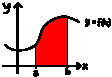
\includegraphics[width=4cm]{2020-1-C2/area-intro-1.pdf}}
  \right)
$$

\newpage

$$\Intx{a}{b}{f(x)} = \Area \left(
  \myvcenter{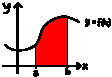
\includegraphics[width=4cm]{2020-1-C2/area-intro-1.pdf}}
  \right)
$$

Pra aprender a calcular essas áreas a gente vai ter que aprender a
aproximá-las por somas de retângulos -- um limite complicado! -- e os
detalhes vão dar um trabalhão... $\frown$

Repare, a área em vermelho é delimitada:

por cima pela \ColorRed{curva} $y=f(x)$,

pela esquerda pela reta $x=a$,

pela direita pela reta $x=b$,

por baixo pela reta $y=0$.

\newpage

% «EDOs»  (to ".EDOs")
% (c2m202introp 4 "EDOs")
% (c2m202introa   "EDOs")

{\bf Equações diferenciais} (lembre: ``ordinárias'' $→$ ``EDOs'') são
um pouco mais complicadas do que as equações que já sabemos
resolver...

\def\te{\text}

\msk

$\scalebox{0.90}{$
\begin{array}{rll}
 1) & x+2   = 5                   & \te{Equação de 1º grau} \\
 2) & x^2+3 = 7                   & \te{Eq.\ de 2º grau simples} \\
 3) & x^2+x = 6                   & \te{Eq.\ de 2º grau mais complicada} \\[5pt]
 4) & f'(x) = x^4                 & \te{EDO simples} \\
    & \text{ou: } \ddx f(x) = x^4 & \te{$f$ é a váriavel/incógnita!!!} \\
 5) & f'(x) = 2f(x)               & \te{EDO mais complicada} \\
 6) & f''(x) + f'(x) = 6f(x)      & \te{idem} \\
 7) & f'(x) = -1/f(x)             & \te{idem} \\
 8) & f'(x) = -x/f(x)             & \te{idem} \\
 \end{array}
 $}
$

\msk

Na passagem de (1) para (2) e (3) as equações ficaram mais complicadas
porque o $x$ passou a poder aparecer elevado ao quadrado.

No (4) estamos procurando uma \ColorRed{função} $f:\R→\R$ que obedeça
$f'(x) = x^4$ \ColorRed{para todo $x$}. Esse ``para todo $x$'' fica
\ColorRed{implícito}.

\newpage

% «chutar-e-testar»  (to ".chutar-e-testar")
% (c2m202introp 5 "chutar-e-testar")
% (c2m202introa   "chutar-e-testar")

{\bf Chutar e testar}

Nosso primeiro método de resolver equações vai ser \ColorRed{chutar e
  testar} -- nós vamos chutar valores pra incógnita e ver se algum
deles é uma solução.

\begin{center}

\bf\Large

Aprender a \ColorRed{testar} vai ser
\underline{\underline{\underline{A}}} coisa

mais importante do curso.

\end{center}

\newpage

Neste curso nós vamos usar quatro coisas que não são padrão

em cursos de Cálculo 2:

\begin{enumerate}

\item A operação `$[:=]$' para substituição de variáveis em

  expressões arbitrárias (veja
  \href{http://angg.twu.net/LATEX/2021-1-C2-subst.pdf}{este PDF}),

\item Às vezes vamos usar `$=$'s na vertical: `$\rotl{=}$',

\item Às vezes vamos definir funções usando gráficos,

\item Nós vamos usar a fórmula $e^{iθ} = \cosθ + i\senθ$ a beça.

\end{enumerate}

\newpage

% «exercicio-1»  (to ".exercicio-1")
% (c2m211introp 7 "exercicio-1")
% (c2m211introa   "exercicio-1")

{\bf Exercício}

Tente resolver as EDOs abaixo (de um dos primeiros slides) por chutar
e testar.

$$\begin{array}{rll}
 4) & f'(x) = x^4                 & \te{EDO simples} \\
    & \text{ou: } \ddx f(x) = x^4 & \te{$f$ é a váriavel/incógnita!!!} \\
 5) & f'(x) = 2f(x)               & \te{EDO mais complicada} \\
 6) & f''(x) + f'(x) = 6f(x)      & \te{idem} \\
 7) & f'(x) = -1/f(x)             & \te{idem} \\
 8) & f'(x) = -x/f(x)             & \te{idem} \\
 \end{array}
$$

Sugestão: comece testando $f(x) = x^3$, $f(x) = x^5$, $f(x) = 200x^5 +
42$, $f(x) = e^x$, $f(x) = e^{42x}$, $f(x) = e^{2x}$, $f(x)=e^{3x}$,
$f(x) = \sqrt{1-x^2}$, $f(x) = \sqrt{4-x^2}$.






%\printbibliography

\GenericWarning{Success:}{Success!!!}  % Used by `M-x cv'

\end{document}

%  ____  _             _         
% |  _ \(_)_   ___   _(_)_______ 
% | | | | \ \ / / | | | |_  / _ \
% | |_| | |\ V /| |_| | |/ /  __/
% |____// | \_/  \__,_|_/___\___|
%     |__/                       
%
% «djvuize»  (to ".djvuize")
% (find-LATEXgrep "grep --color -nH --null -e djvuize 2020-1*.tex")

 (eepitch-shell)
 (eepitch-kill)
 (eepitch-shell)
# (find-fline "~/2021.1-C2/")
# (find-fline "~/LATEX/2021-1-C2/")
# (find-fline "~/bin/djvuize")

cd /tmp/
for i in *.jpg; do echo f $(basename $i .jpg); done

f () { rm -fv $1.png $1.pdf; djvuize $1.pdf }
f () { rm -fv $1.png $1.pdf; djvuize WHITEBOARDOPTS="-m 1.0" $1.pdf; xpdf $1.pdf }
f () { rm -fv $1.png $1.pdf; djvuize WHITEBOARDOPTS="-m 0.5" $1.pdf; xpdf $1.pdf }
f () { rm -fv $1.png $1.pdf; djvuize WHITEBOARDOPTS="-m 0.25" $1.pdf; xpdf $1.pdf }
f () { cp -fv $1.png $1.pdf       ~/2021.1-C2/
       cp -fv        $1.pdf ~/LATEX/2021-1-C2/
       cat <<%%%
% (find-latexscan-links "C2" "$1")
%%%
}

f 20201213_area_em_funcao_de_theta
f 20201213_area_em_funcao_de_x
f 20201213_area_fatias_pizza



%  __  __       _        
% |  \/  | __ _| | _____ 
% | |\/| |/ _` | |/ / _ \
% | |  | | (_| |   <  __/
% |_|  |_|\__,_|_|\_\___|
%                        
% <make>

 (eepitch-shell)
 (eepitch-kill)
 (eepitch-shell)
# (find-LATEXfile "2019planar-has-1.mk")
make -f 2019.mk STEM=2021-1-C2-intro veryclean
make -f 2019.mk STEM=2021-1-C2-intro pdf

% Local Variables:
% coding: utf-8-unix
% ee-tla: "c2m211intro"
% End:
